\documentclass[1p]{elsarticle_modified}
%\bibliographystyle{elsarticle-num}

%\usepackage[colorlinks]{hyperref}
%\usepackage{abbrmath_seonhwa} %\Abb, \Ascr, \Acal ,\Abf, \Afrak
\usepackage{amsfonts}
\usepackage{amssymb}
\usepackage{amsmath}
\usepackage{amsthm}
\usepackage{scalefnt}
\usepackage{amsbsy}
\usepackage{kotex}
\usepackage{caption}
\usepackage{subfig}
\usepackage{color}
\usepackage{graphicx}
\usepackage{xcolor} %% white, black, red, green, blue, cyan, magenta, yellow
\usepackage{float}
\usepackage{setspace}
\usepackage{hyperref}

\usepackage{tikz}
\usetikzlibrary{arrows}

\usepackage{multirow}
\usepackage{array} % fixed length table
\usepackage{hhline}

%%%%%%%%%%%%%%%%%%%%%
\makeatletter
\renewcommand*\env@matrix[1][\arraystretch]{%
	\edef\arraystretch{#1}%
	\hskip -\arraycolsep
	\let\@ifnextchar\new@ifnextchar
	\array{*\c@MaxMatrixCols c}}
\makeatother %https://tex.stackexchange.com/questions/14071/how-can-i-increase-the-line-spacing-in-a-matrix
%%%%%%%%%%%%%%%

\usepackage[normalem]{ulem}

\newcommand{\msout}[1]{\ifmmode\text{\sout{\ensuremath{#1}}}\else\sout{#1}\fi}
%SOURCE: \msout is \stkout macro in https://tex.stackexchange.com/questions/20609/strikeout-in-math-mode

\newcommand{\cancel}[1]{
	\ifmmode
	{\color{red}\msout{#1}}
	\else
	{\color{red}\sout{#1}}
	\fi
}

\newcommand{\add}[1]{
	{\color{blue}\uwave{#1}}
}

\newcommand{\replace}[2]{
	\ifmmode
	{\color{red}\msout{#1}}{\color{blue}\uwave{#2}}
	\else
	{\color{red}\sout{#1}}{\color{blue}\uwave{#2}}
	\fi
}

\newcommand{\Sol}{\mathcal{S}} %segment
\newcommand{\D}{D} %diagram
\newcommand{\A}{\mathcal{A}} %arc


%%%%%%%%%%%%%%%%%%%%%%%%%%%%%5 test

\def\sl{\operatorname{\textup{SL}}(2,\Cbb)}
\def\psl{\operatorname{\textup{PSL}}(2,\Cbb)}
\def\quan{\mkern 1mu \triangleright \mkern 1mu}

\theoremstyle{definition}
\newtheorem{thm}{Theorem}[section]
\newtheorem{prop}[thm]{Proposition}
\newtheorem{lem}[thm]{Lemma}
\newtheorem{ques}[thm]{Question}
\newtheorem{cor}[thm]{Corollary}
\newtheorem{defn}[thm]{Definition}
\newtheorem{exam}[thm]{Example}
\newtheorem{rmk}[thm]{Remark}
\newtheorem{alg}[thm]{Algorithm}

\newcommand{\I}{\sqrt{-1}}
\begin{document}

%\begin{frontmatter}
%
%\title{Boundary parabolic representations of knots up to 8 crossings}
%
%%% Group authors per affiliation:
%\author{Yunhi Cho} 
%\address{Department of Mathematics, University of Seoul, Seoul, Korea}
%\ead{yhcho@uos.ac.kr}
%
%
%\author{Seonhwa Kim} %\fnref{s_kim}}
%\address{Center for Geometry and Physics, Institute for Basic Science, Pohang, 37673, Korea}
%\ead{ryeona17@ibs.re.kr}
%
%\author{Hyuk Kim}
%\address{Department of Mathematical Sciences, Seoul National University, Seoul 08826, Korea}
%\ead{hyukkim@snu.ac.kr}
%
%\author{Seokbeom Yoon}
%\address{Department of Mathematical Sciences, Seoul National University, Seoul, 08826,  Korea}
%\ead{sbyoon15@snu.ac.kr}
%
%\begin{abstract}
%We find all boundary parabolic representation of knots up to 8 crossings.
%
%\end{abstract}
%\begin{keyword}
%    \MSC[2010] 57M25 
%\end{keyword}
%
%\end{frontmatter}

%\linenumbers
%\tableofcontents
%
\newcommand\colored[1]{\textcolor{white}{\rule[-0.35ex]{0.8em}{1.4ex}}\kern-0.8em\color{red} #1}%
%\newcommand\colored[1]{\textcolor{white}{ #1}\kern-2.17ex	\textcolor{white}{ #1}\kern-1.81ex	\textcolor{white}{ #1}\kern-2.15ex\color{red}#1	}

{\Large $\underline{12a_{1036}~(K12a_{1036})}$}

\setlength{\tabcolsep}{10pt}
\renewcommand{\arraystretch}{1.6}
\vspace{1cm}\begin{tabular}{m{100pt}>{\centering\arraybackslash}m{274pt}}
\multirow{5}{120pt}{
	\centering
	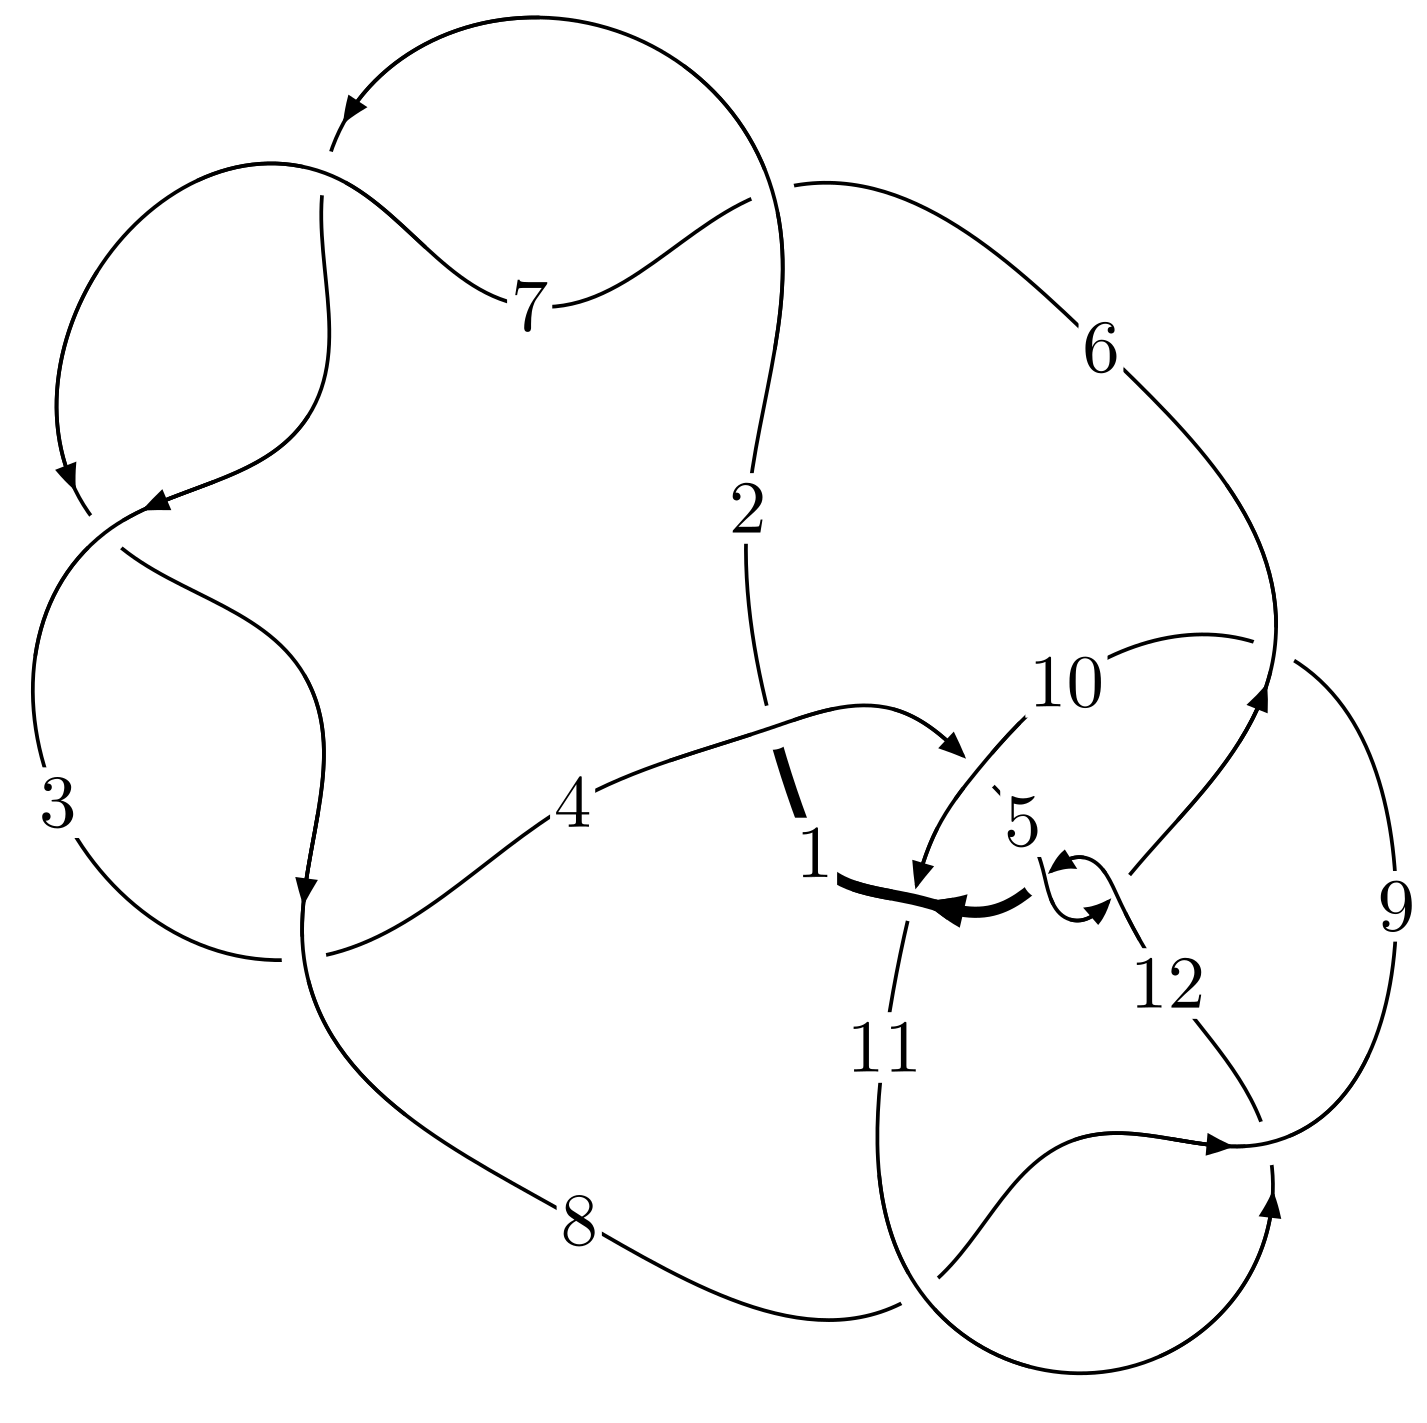
\includegraphics[width=112pt]{../../../GIT/diagram.site/Diagrams/png/1837_12a_1036.png}\\
\ \ \ A knot diagram\footnotemark}&
\allowdisplaybreaks
\textbf{Linearized knot diagam} \\
\cline{2-2}
 &
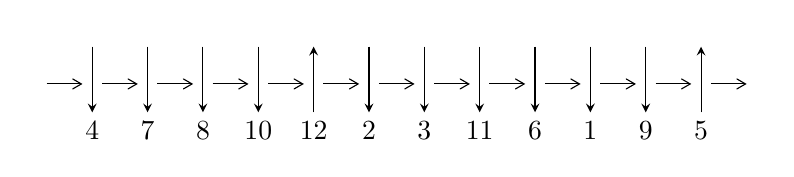
\begin{tikzpicture}[x=20pt, y=17pt]
	% nodes
	\node (C0) at (0, 0) {};
	\node (C1) at (1, 0) {};
	\node (C1U) at (1, +1) {};
	\node (C1D) at (1, -1) {4};

	\node (C2) at (2, 0) {};
	\node (C2U) at (2, +1) {};
	\node (C2D) at (2, -1) {7};

	\node (C3) at (3, 0) {};
	\node (C3U) at (3, +1) {};
	\node (C3D) at (3, -1) {8};

	\node (C4) at (4, 0) {};
	\node (C4U) at (4, +1) {};
	\node (C4D) at (4, -1) {10};

	\node (C5) at (5, 0) {};
	\node (C5U) at (5, +1) {};
	\node (C5D) at (5, -1) {12};

	\node (C6) at (6, 0) {};
	\node (C6U) at (6, +1) {};
	\node (C6D) at (6, -1) {2};

	\node (C7) at (7, 0) {};
	\node (C7U) at (7, +1) {};
	\node (C7D) at (7, -1) {3};

	\node (C8) at (8, 0) {};
	\node (C8U) at (8, +1) {};
	\node (C8D) at (8, -1) {11};

	\node (C9) at (9, 0) {};
	\node (C9U) at (9, +1) {};
	\node (C9D) at (9, -1) {6};

	\node (C10) at (10, 0) {};
	\node (C10U) at (10, +1) {};
	\node (C10D) at (10, -1) {1};

	\node (C11) at (11, 0) {};
	\node (C11U) at (11, +1) {};
	\node (C11D) at (11, -1) {9};

	\node (C12) at (12, 0) {};
	\node (C12U) at (12, +1) {};
	\node (C12D) at (12, -1) {5};
	\node (C13) at (13, 0) {};

	% arrows
	\draw[->,>={angle 60}]
	(C0) edge (C1) (C1) edge (C2) (C2) edge (C3) (C3) edge (C4) (C4) edge (C5) (C5) edge (C6) (C6) edge (C7) (C7) edge (C8) (C8) edge (C9) (C9) edge (C10) (C10) edge (C11) (C11) edge (C12) (C12) edge (C13) ;	\draw[->,>=stealth]
	(C1U) edge (C1D) (C2U) edge (C2D) (C3U) edge (C3D) (C4U) edge (C4D) (C5D) edge (C5U) (C6U) edge (C6D) (C7U) edge (C7D) (C8U) edge (C8D) (C9U) edge (C9D) (C10U) edge (C10D) (C11U) edge (C11D) (C12D) edge (C12U) ;
	\end{tikzpicture} \\
\hhline{~~} \\& 
\textbf{Solving Sequence} \\ \cline{2-2} 
 &
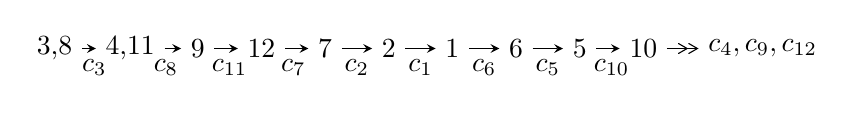
\begin{tikzpicture}[x=23pt, y=7pt]
	% node
	\node (A0) at (-1/8, 0) {3,8};
	\node (A1) at (17/16, 0) {4,11};
	\node (A2) at (17/8, 0) {9};
	\node (A3) at (25/8, 0) {12};
	\node (A4) at (33/8, 0) {7};
	\node (A5) at (41/8, 0) {2};
	\node (A6) at (49/8, 0) {1};
	\node (A7) at (57/8, 0) {6};
	\node (A8) at (65/8, 0) {5};
	\node (A9) at (73/8, 0) {10};
	\node (C1) at (1/2, -1) {$c_{3}$};
	\node (C2) at (13/8, -1) {$c_{8}$};
	\node (C3) at (21/8, -1) {$c_{11}$};
	\node (C4) at (29/8, -1) {$c_{7}$};
	\node (C5) at (37/8, -1) {$c_{2}$};
	\node (C6) at (45/8, -1) {$c_{1}$};
	\node (C7) at (53/8, -1) {$c_{6}$};
	\node (C8) at (61/8, -1) {$c_{5}$};
	\node (C9) at (69/8, -1) {$c_{10}$};
	\node (A10) at (11, 0) {$c_{4},c_{9},c_{12}$};

	% edge
	\draw[->,>=stealth]	
	(A0) edge (A1) (A1) edge (A2) (A2) edge (A3) (A3) edge (A4) (A4) edge (A5) (A5) edge (A6) (A6) edge (A7) (A7) edge (A8) (A8) edge (A9) ;
	\draw[->>,>={angle 60}]	
	(A9) edge (A10);
\end{tikzpicture} \\ 

\end{tabular} \\

\footnotetext{
The image of knot diagram is generated by the software ``\textbf{Draw programme}" developed by Andrew Bartholomew(\url{http://www.layer8.co.uk/maths/draw/index.htm\#Running-draw}), where we modified some parts for our purpose(\url{https://github.com/CATsTAILs/LinksPainter}).
}\phantom \\ \newline 
\centering \textbf{Ideals for irreducible components\footnotemark of $X_{\text{par}}$} 
 
\begin{align*}
I^u_{1}&=\langle 
1.00424\times10^{43} u^{79}+4.59153\times10^{43} u^{78}+\cdots+3.52066\times10^{43} b-2.24988\times10^{43},\\
\phantom{I^u_{1}}&\phantom{= \langle  }2.59495\times10^{43} u^{79}+5.15203\times10^{43} u^{78}+\cdots+1.76033\times10^{43} a+4.42143\times10^{43},\;u^{80}+2 u^{79}+\cdots+3 u-1\rangle \\
I^u_{2}&=\langle 
2 b+3,\;a+1,\;u-1\rangle \\
\\
\end{align*}
\raggedright * 2 irreducible components of $\dim_{\mathbb{C}}=0$, with total 81 representations.\\
\footnotetext{All coefficients of polynomials are rational numbers. But the coefficients are sometimes approximated in decimal forms when there is not enough margin.}
\newpage
\renewcommand{\arraystretch}{1}
\centering \section*{I. $I^u_{1}= \langle 1.00\times10^{43} u^{79}+4.59\times10^{43} u^{78}+\cdots+3.52\times10^{43} b-2.25\times10^{43},\;2.59\times10^{43} u^{79}+5.15\times10^{43} u^{78}+\cdots+1.76\times10^{43} a+4.42\times10^{43},\;u^{80}+2 u^{79}+\cdots+3 u-1 \rangle$}
\flushleft \textbf{(i) Arc colorings}\\
\begin{tabular}{m{7pt} m{180pt} m{7pt} m{180pt} }
\flushright $a_{3}=$&$\begin{pmatrix}1\\0\end{pmatrix}$ \\
\flushright $a_{8}=$&$\begin{pmatrix}0\\u\end{pmatrix}$ \\
\flushright $a_{4}=$&$\begin{pmatrix}1\\u^2\end{pmatrix}$ \\
\flushright $a_{11}=$&$\begin{pmatrix}-1.47413 u^{79}-2.92674 u^{78}+\cdots+2.87021 u-2.51170\\-0.285241 u^{79}-1.30417 u^{78}+\cdots-0.132168 u+0.639050\end{pmatrix}$ \\
\flushright $a_{9}=$&$\begin{pmatrix}-1.19118 u^{79}-2.62336 u^{78}+\cdots+4.64115 u-2.35738\\-0.0380110 u^{79}-1.07750 u^{78}+\cdots+1.66477 u+0.484932\end{pmatrix}$ \\
\flushright $a_{12}=$&$\begin{pmatrix}-0.672774 u^{79}-0.857234 u^{78}+\cdots-2.79688 u-0.488433\\-0.356975 u^{79}-0.458287 u^{78}+\cdots-1.89586 u+0.215000\end{pmatrix}$ \\
\flushright $a_{7}=$&$\begin{pmatrix}u\\u\end{pmatrix}$ \\
\flushright $a_{2}=$&$\begin{pmatrix}- u^2+1\\- u^2\end{pmatrix}$ \\
\flushright $a_{1}=$&$\begin{pmatrix}u^4-3 u^2+1\\u^6-2 u^4- u^2\end{pmatrix}$ \\
\flushright $a_{6}=$&$\begin{pmatrix}- u^3+2 u\\- u^3+u\end{pmatrix}$ \\
\flushright $a_{5}=$&$\begin{pmatrix}-0.273315 u^{79}-0.539846 u^{78}+\cdots+1.40791 u-0.578088\\-0.900556 u^{79}-0.871675 u^{78}+\cdots-1.82355 u+0.679557\end{pmatrix}$ \\
\flushright $a_{10}=$&$\begin{pmatrix}-1.05861 u^{79}-0.640733 u^{78}+\cdots+0.478677 u-1.55838\\-1.31826 u^{79}-0.626854 u^{78}+\cdots-3.06336 u+1.53127\end{pmatrix}$\\&\end{tabular}
\flushleft \textbf{(ii) Obstruction class $= -1$}\\~\\
\flushleft \textbf{(iii) Cusp Shapes $= -0.998004 u^{79}-3.77601 u^{78}+\cdots-4.55085 u-10.1964$}\\~\\
\newpage\renewcommand{\arraystretch}{1}
\flushleft \textbf{(iv) u-Polynomials at the component}\newline \\
\begin{tabular}{m{50pt}|m{274pt}}
Crossings & \hspace{64pt}u-Polynomials at each crossing \\
\hline $$\begin{aligned}c_{1}\end{aligned}$$&$\begin{aligned}
&u^{80}-18 u^{79}+\cdots+12967 u-1633
\end{aligned}$\\
\hline $$\begin{aligned}c_{2},c_{3},c_{6}\\c_{7}\end{aligned}$$&$\begin{aligned}
&u^{80}-2 u^{79}+\cdots-3 u-1
\end{aligned}$\\
\hline $$\begin{aligned}c_{4}\end{aligned}$$&$\begin{aligned}
&u^{80}- u^{79}+\cdots-22 u+8
\end{aligned}$\\
\hline $$\begin{aligned}c_{5},c_{12}\end{aligned}$$&$\begin{aligned}
&u^{80}-2 u^{79}+\cdots- u-1
\end{aligned}$\\
\hline $$\begin{aligned}c_{8},c_{11}\end{aligned}$$&$\begin{aligned}
&u^{80}-2 u^{79}+\cdots-105 u-4
\end{aligned}$\\
\hline $$\begin{aligned}c_{9}\end{aligned}$$&$\begin{aligned}
&2(2 u^{80}+17 u^{79}+\cdots+668890 u+195281)
\end{aligned}$\\
\hline $$\begin{aligned}c_{10}\end{aligned}$$&$\begin{aligned}
&2(2 u^{80}- u^{79}+\cdots+37298 u-1559)
\end{aligned}$\\
\hline
\end{tabular}\\~\\
\newpage\renewcommand{\arraystretch}{1}
\flushleft \textbf{(v) Riley Polynomials at the component}\newline \\
\begin{tabular}{m{50pt}|m{274pt}}
Crossings & \hspace{64pt}Riley Polynomials at each crossing \\
\hline $$\begin{aligned}c_{1}\end{aligned}$$&$\begin{aligned}
&y^{80}+6 y^{79}+\cdots+33342983 y+2666689
\end{aligned}$\\
\hline $$\begin{aligned}c_{2},c_{3},c_{6}\\c_{7}\end{aligned}$$&$\begin{aligned}
&y^{80}-90 y^{79}+\cdots-9 y+1
\end{aligned}$\\
\hline $$\begin{aligned}c_{4}\end{aligned}$$&$\begin{aligned}
&y^{80}-9 y^{79}+\cdots-3892 y+64
\end{aligned}$\\
\hline $$\begin{aligned}c_{5},c_{12}\end{aligned}$$&$\begin{aligned}
&y^{80}+58 y^{79}+\cdots-9 y+1
\end{aligned}$\\
\hline $$\begin{aligned}c_{8},c_{11}\end{aligned}$$&$\begin{aligned}
&y^{80}-58 y^{79}+\cdots-2705 y+16
\end{aligned}$\\
\hline $$\begin{aligned}c_{9}\end{aligned}$$&$\begin{aligned}
&4(4 y^{80}-413 y^{79}+\cdots-9.97980\times10^{11} y+3.81347\times10^{10})
\end{aligned}$\\
\hline $$\begin{aligned}c_{10}\end{aligned}$$&$\begin{aligned}
&4(4 y^{80}+179 y^{79}+\cdots-4.44111\times10^{8} y+2430481)
\end{aligned}$\\
\hline
\end{tabular}\\~\\
\newpage\flushleft \textbf{(vi) Complex Volumes and Cusp Shapes}
$$\begin{array}{c|c|c}  
\text{Solutions to }I^u_{1}& \I (\text{vol} + \sqrt{-1}CS) & \text{Cusp shape}\\
 \hline 
\begin{aligned}
u &= \phantom{-}0.710776 + 0.643207 I \\
a &= \phantom{-}0.885948 - 0.811257 I \\
b &= \phantom{-}1.183380 - 0.325061 I\end{aligned}
 & -4.80399 - 1.23940 I & \phantom{-0.000000 } 0 \\ \hline\begin{aligned}
u &= \phantom{-}0.710776 - 0.643207 I \\
a &= \phantom{-}0.885948 + 0.811257 I \\
b &= \phantom{-}1.183380 + 0.325061 I\end{aligned}
 & -4.80399 + 1.23940 I & \phantom{-0.000000 } 0 \\ \hline\begin{aligned}
u &= -1.071960 + 0.150156 I \\
a &= -1.167190 - 0.522833 I \\
b &= -1.59214 - 0.23719 I\end{aligned}
 & -8.96202 - 6.56324 I & \phantom{-0.000000 } 0 \\ \hline\begin{aligned}
u &= -1.071960 - 0.150156 I \\
a &= -1.167190 + 0.522833 I \\
b &= -1.59214 + 0.23719 I\end{aligned}
 & -8.96202 + 6.56324 I & \phantom{-0.000000 } 0 \\ \hline\begin{aligned}
u &= -0.710675 + 0.561732 I \\
a &= -1.317040 - 0.460428 I \\
b &= -1.77036 - 0.25799 I\end{aligned}
 & -1.10749 + 8.10126 I & \phantom{-0.000000 } 0 \\ \hline\begin{aligned}
u &= -0.710675 - 0.561732 I \\
a &= -1.317040 + 0.460428 I \\
b &= -1.77036 + 0.25799 I\end{aligned}
 & -1.10749 - 8.10126 I & \phantom{-0.000000 } 0 \\ \hline\begin{aligned}
u &= \phantom{-}0.690803 + 0.566225 I \\
a &= \phantom{-}1.61403 - 0.52729 I \\
b &= \phantom{-}1.99838 - 0.45165 I\end{aligned}
 & -6.0204 - 13.6937 I & \phantom{-0.000000 } 0 \\ \hline\begin{aligned}
u &= \phantom{-}0.690803 - 0.566225 I \\
a &= \phantom{-}1.61403 + 0.52729 I \\
b &= \phantom{-}1.99838 + 0.45165 I\end{aligned}
 & -6.0204 + 13.6937 I & \phantom{-0.000000 } 0 \\ \hline\begin{aligned}
u &= \phantom{-}1.087620 + 0.310670 I \\
a &= \phantom{-}0.871693 - 0.378049 I \\
b &= \phantom{-}1.52235 - 0.10204 I\end{aligned}
 & -3.59474 + 0.54452 I & \phantom{-0.000000 } 0 \\ \hline\begin{aligned}
u &= \phantom{-}1.087620 - 0.310670 I \\
a &= \phantom{-}0.871693 + 0.378049 I \\
b &= \phantom{-}1.52235 + 0.10204 I\end{aligned}
 & -3.59474 - 0.54452 I & \phantom{-0.000000 } 0\\
 \hline 
 \end{array}$$\newpage$$\begin{array}{c|c|c}  
\text{Solutions to }I^u_{1}& \I (\text{vol} + \sqrt{-1}CS) & \text{Cusp shape}\\
 \hline 
\begin{aligned}
u &= \phantom{-}0.633761 + 0.498635 I \\
a &= -1.03703 - 1.17829 I \\
b &= -0.977072 - 0.435927 I\end{aligned}
 & -1.33572 - 7.46742 I & -11.1826 + 9.5153 I \\ \hline\begin{aligned}
u &= \phantom{-}0.633761 - 0.498635 I \\
a &= -1.03703 + 1.17829 I \\
b &= -0.977072 + 0.435927 I\end{aligned}
 & -1.33572 + 7.46742 I & -11.1826 - 9.5153 I \\ \hline\begin{aligned}
u &= \phantom{-}0.318682 + 0.726773 I \\
a &= \phantom{-}0.73666 - 1.24121 I \\
b &= \phantom{-}0.293019 - 0.055818 I\end{aligned}
 & -3.65149 - 3.40355 I & -15.8663 + 9.7793 I \\ \hline\begin{aligned}
u &= \phantom{-}0.318682 - 0.726773 I \\
a &= \phantom{-}0.73666 + 1.24121 I \\
b &= \phantom{-}0.293019 + 0.055818 I\end{aligned}
 & -3.65149 + 3.40355 I & -15.8663 - 9.7793 I \\ \hline\begin{aligned}
u &= -0.599259 + 0.512610 I \\
a &= \phantom{-}0.482290 - 0.886004 I \\
b &= \phantom{-}0.411608 - 0.215285 I\end{aligned}
 & \phantom{-}2.07455 + 3.71807 I & -4.86829 - 5.38246 I \\ \hline\begin{aligned}
u &= -0.599259 - 0.512610 I \\
a &= \phantom{-}0.482290 + 0.886004 I \\
b &= \phantom{-}0.411608 + 0.215285 I\end{aligned}
 & \phantom{-}2.07455 - 3.71807 I & -4.86829 + 5.38246 I \\ \hline\begin{aligned}
u &= -0.654476 + 0.408860 I \\
a &= \phantom{-}2.13802 + 0.15533 I \\
b &= \phantom{-}1.89759 + 0.54937 I\end{aligned}
 & -6.07316 + 4.58559 I & -17.4937 - 8.2107 I \\ \hline\begin{aligned}
u &= -0.654476 - 0.408860 I \\
a &= \phantom{-}2.13802 - 0.15533 I \\
b &= \phantom{-}1.89759 - 0.54937 I\end{aligned}
 & -6.07316 - 4.58559 I & -17.4937 + 8.2107 I \\ \hline\begin{aligned}
u &= \phantom{-}0.600089 + 0.409057 I \\
a &= -1.43887 + 0.37749 I \\
b &= -1.75891 + 0.90980 I\end{aligned}
 & -1.82378 - 2.98170 I & -10.11561 + 6.06219 I \\ \hline\begin{aligned}
u &= \phantom{-}0.600089 - 0.409057 I \\
a &= -1.43887 - 0.37749 I \\
b &= -1.75891 - 0.90980 I\end{aligned}
 & -1.82378 + 2.98170 I & -10.11561 - 6.06219 I\\
 \hline 
 \end{array}$$\newpage$$\begin{array}{c|c|c}  
\text{Solutions to }I^u_{1}& \I (\text{vol} + \sqrt{-1}CS) & \text{Cusp shape}\\
 \hline 
\begin{aligned}
u &= \phantom{-}0.663019 + 0.295461 I \\
a &= -1.85860 + 1.35693 I \\
b &= -1.23197 + 0.84021 I\end{aligned}
 & -6.77446 - 0.42985 I & -19.7000 + 2.6791 I \\ \hline\begin{aligned}
u &= \phantom{-}0.663019 - 0.295461 I \\
a &= -1.85860 - 1.35693 I \\
b &= -1.23197 - 0.84021 I\end{aligned}
 & -6.77446 + 0.42985 I & -19.7000 - 2.6791 I \\ \hline\begin{aligned}
u &= \phantom{-}0.560189 + 0.430465 I \\
a &= -0.088937 + 0.123185 I \\
b &= \phantom{-}0.438182 + 0.745626 I\end{aligned}
 & -1.57329 - 1.33652 I & -10.84600 + 4.10196 I \\ \hline\begin{aligned}
u &= \phantom{-}0.560189 - 0.430465 I \\
a &= -0.088937 - 0.123185 I \\
b &= \phantom{-}0.438182 - 0.745626 I\end{aligned}
 & -1.57329 + 1.33652 I & -10.84600 - 4.10196 I \\ \hline\begin{aligned}
u &= -0.202836 + 0.676160 I \\
a &= \phantom{-}0.03227 - 1.63491 I \\
b &= \phantom{-}0.135199 + 0.115033 I\end{aligned}
 & \phantom{-}0.39318 - 3.94675 I & -7.46064 + 5.59144 I \\ \hline\begin{aligned}
u &= -0.202836 - 0.676160 I \\
a &= \phantom{-}0.03227 + 1.63491 I \\
b &= \phantom{-}0.135199 - 0.115033 I\end{aligned}
 & \phantom{-}0.39318 + 3.94675 I & -7.46064 - 5.59144 I \\ \hline\begin{aligned}
u &= \phantom{-}0.239815 + 0.662724 I \\
a &= -0.02247 - 2.06927 I \\
b &= -0.277197 - 0.045286 I\end{aligned}
 & -4.68567 + 9.55045 I & -10.51022 - 4.70720 I \\ \hline\begin{aligned}
u &= \phantom{-}0.239815 - 0.662724 I \\
a &= -0.02247 + 2.06927 I \\
b &= -0.277197 + 0.045286 I\end{aligned}
 & -4.68567 - 9.55045 I & -10.51022 + 4.70720 I \\ \hline\begin{aligned}
u &= -1.304910 + 0.149597 I \\
a &= -0.938271 + 0.143542 I \\
b &= -1.56342 - 0.08918 I\end{aligned}
 & -8.74851 + 6.64165 I & \phantom{-0.000000 } 0 \\ \hline\begin{aligned}
u &= -1.304910 - 0.149597 I \\
a &= -0.938271 - 0.143542 I \\
b &= -1.56342 + 0.08918 I\end{aligned}
 & -8.74851 - 6.64165 I & \phantom{-0.000000 } 0\\
 \hline 
 \end{array}$$\newpage$$\begin{array}{c|c|c}  
\text{Solutions to }I^u_{1}& \I (\text{vol} + \sqrt{-1}CS) & \text{Cusp shape}\\
 \hline 
\begin{aligned}
u &= -0.673205 + 0.061428 I \\
a &= \phantom{-}0.557215 + 1.268730 I \\
b &= -0.343363 + 0.602925 I\end{aligned}
 & -3.81684 - 2.51015 I & -16.7147 + 3.2878 I \\ \hline\begin{aligned}
u &= -0.673205 - 0.061428 I \\
a &= \phantom{-}0.557215 - 1.268730 I \\
b &= -0.343363 - 0.602925 I\end{aligned}
 & -3.81684 + 2.51015 I & -16.7147 - 3.2878 I \\ \hline\begin{aligned}
u &= -0.564500 + 0.320140 I \\
a &= \phantom{-}1.47412 + 0.99082 I \\
b &= \phantom{-}1.56072 - 0.33590 I\end{aligned}
 & -2.47702 + 1.06134 I & -6.54054 - 7.20108 I \\ \hline\begin{aligned}
u &= -0.564500 - 0.320140 I \\
a &= \phantom{-}1.47412 - 0.99082 I \\
b &= \phantom{-}1.56072 + 0.33590 I\end{aligned}
 & -2.47702 - 1.06134 I & -6.54054 + 7.20108 I \\ \hline\begin{aligned}
u &= -0.338597 + 0.546034 I \\
a &= -1.121980 + 0.163936 I \\
b &= -0.643789 + 0.047876 I\end{aligned}
 & \phantom{-}2.83880 - 0.05741 I & -2.05176 - 2.16439 I \\ \hline\begin{aligned}
u &= -0.338597 - 0.546034 I \\
a &= -1.121980 - 0.163936 I \\
b &= -0.643789 - 0.047876 I\end{aligned}
 & \phantom{-}2.83880 + 0.05741 I & -2.05176 + 2.16439 I \\ \hline\begin{aligned}
u &= -0.471894 + 0.402538 I \\
a &= \phantom{-}1.24902 + 1.00105 I \\
b &= -5.06449 + 0.31875 I\end{aligned}
 & -3.05065 + 1.47279 I & -24.2014 + 56.8592 I \\ \hline\begin{aligned}
u &= -0.471894 - 0.402538 I \\
a &= \phantom{-}1.24902 - 1.00105 I \\
b &= -5.06449 - 0.31875 I\end{aligned}
 & -3.05065 - 1.47279 I & -24.2014 - 56.8592 I \\ \hline\begin{aligned}
u &= \phantom{-}0.274551 + 0.532663 I \\
a &= \phantom{-}1.62148 + 0.87755 I \\
b &= \phantom{-}0.821167 + 0.129127 I\end{aligned}
 & -0.29599 + 3.88984 I & -7.52657 - 3.20009 I \\ \hline\begin{aligned}
u &= \phantom{-}0.274551 - 0.532663 I \\
a &= \phantom{-}1.62148 - 0.87755 I \\
b &= \phantom{-}0.821167 - 0.129127 I\end{aligned}
 & -0.29599 - 3.88984 I & -7.52657 + 3.20009 I\\
 \hline 
 \end{array}$$\newpage$$\begin{array}{c|c|c}  
\text{Solutions to }I^u_{1}& \I (\text{vol} + \sqrt{-1}CS) & \text{Cusp shape}\\
 \hline 
\begin{aligned}
u &= \phantom{-}1.43956 + 0.08554 I \\
a &= \phantom{-}0.402543 + 0.391723 I \\
b &= \phantom{-}1.356760 - 0.062941 I\end{aligned}
 & -2.80082 - 2.02963 I & \phantom{-0.000000 } 0 \\ \hline\begin{aligned}
u &= \phantom{-}1.43956 - 0.08554 I \\
a &= \phantom{-}0.402543 - 0.391723 I \\
b &= \phantom{-}1.356760 + 0.062941 I\end{aligned}
 & -2.80082 + 2.02963 I & \phantom{-0.000000 } 0 \\ \hline\begin{aligned}
u &= -1.46069 + 0.03248 I \\
a &= -0.184564 + 0.602641 I \\
b &= -1.365120 + 0.065647 I\end{aligned}
 & -5.60735 - 2.30773 I & \phantom{-0.000000 } 0 \\ \hline\begin{aligned}
u &= -1.46069 - 0.03248 I \\
a &= -0.184564 - 0.602641 I \\
b &= -1.365120 - 0.065647 I\end{aligned}
 & -5.60735 + 2.30773 I & \phantom{-0.000000 } 0 \\ \hline\begin{aligned}
u &= \phantom{-}0.476315\phantom{ +0.000000I} \\
a &= -0.663294\phantom{ +0.000000I} \\
b &= \phantom{-}0.350154\phantom{ +0.000000I}\end{aligned}
 & -0.838451\phantom{ +0.000000I} & -11.2140\phantom{ +0.000000I} \\ \hline\begin{aligned}
u &= \phantom{-}0.216462 + 0.420429 I \\
a &= -0.604851 - 0.421093 I \\
b &= \phantom{-}0.134724 + 0.520809 I\end{aligned}
 & -0.69298 - 1.54541 I & -5.72121 + 3.62378 I \\ \hline\begin{aligned}
u &= \phantom{-}0.216462 - 0.420429 I \\
a &= -0.604851 + 0.421093 I \\
b &= \phantom{-}0.134724 - 0.520809 I\end{aligned}
 & -0.69298 + 1.54541 I & -5.72121 - 3.62378 I \\ \hline\begin{aligned}
u &= \phantom{-}1.54898 + 0.09118 I \\
a &= -0.574298 + 0.052082 I \\
b &= \phantom{-}0.29424 - 5.06759 I\end{aligned}
 & -9.91410 - 3.08787 I & \phantom{-0.000000 } 0 \\ \hline\begin{aligned}
u &= \phantom{-}1.54898 - 0.09118 I \\
a &= -0.574298 - 0.052082 I \\
b &= \phantom{-}0.29424 + 5.06759 I\end{aligned}
 & -9.91410 + 3.08787 I & \phantom{-0.000000 } 0 \\ \hline\begin{aligned}
u &= -1.55217 + 0.06245 I \\
a &= \phantom{-}0.348266 + 0.379294 I \\
b &= \phantom{-}0.0510261 + 0.0183574 I\end{aligned}
 & -7.65108 + 0.72597 I & \phantom{-0.000000 } 0\\
 \hline 
 \end{array}$$\newpage$$\begin{array}{c|c|c}  
\text{Solutions to }I^u_{1}& \I (\text{vol} + \sqrt{-1}CS) & \text{Cusp shape}\\
 \hline 
\begin{aligned}
u &= -1.55217 - 0.06245 I \\
a &= \phantom{-}0.348266 - 0.379294 I \\
b &= \phantom{-}0.0510261 - 0.0183574 I\end{aligned}
 & -7.65108 - 0.72597 I & \phantom{-0.000000 } 0 \\ \hline\begin{aligned}
u &= -1.55805 + 0.12389 I \\
a &= \phantom{-}0.1199480 - 0.0670336 I \\
b &= -0.904546 + 0.950420 I\end{aligned}
 & -8.71709 + 3.34696 I & \phantom{-0.000000 } 0 \\ \hline\begin{aligned}
u &= -1.55805 - 0.12389 I \\
a &= \phantom{-}0.1199480 + 0.0670336 I \\
b &= -0.904546 - 0.950420 I\end{aligned}
 & -8.71709 - 3.34696 I & \phantom{-0.000000 } 0 \\ \hline\begin{aligned}
u &= \phantom{-}0.292333 + 0.313766 I \\
a &= -0.89591 + 1.77166 I \\
b &= \phantom{-}0.533166 + 0.109441 I\end{aligned}
 & -0.956674 + 0.198529 I & -8.23896 + 1.94124 I \\ \hline\begin{aligned}
u &= \phantom{-}0.292333 - 0.313766 I \\
a &= -0.89591 - 1.77166 I \\
b &= \phantom{-}0.533166 - 0.109441 I\end{aligned}
 & -0.956674 - 0.198529 I & -8.23896 - 1.94124 I \\ \hline\begin{aligned}
u &= \phantom{-}1.57069 + 0.09402 I \\
a &= -0.774131 + 0.123567 I \\
b &= -4.38000 + 0.20219 I\end{aligned}
 & -9.78363 - 2.58458 I & \phantom{-0.000000 } 0 \\ \hline\begin{aligned}
u &= \phantom{-}1.57069 - 0.09402 I \\
a &= -0.774131 - 0.123567 I \\
b &= -4.38000 - 0.20219 I\end{aligned}
 & -9.78363 + 2.58458 I & \phantom{-0.000000 } 0 \\ \hline\begin{aligned}
u &= -0.122168 + 0.406621 I \\
a &= -0.33255 + 3.35354 I \\
b &= -0.425855 + 0.579814 I\end{aligned}
 & -4.64791 - 1.68703 I & -12.27481 + 1.77640 I \\ \hline\begin{aligned}
u &= -0.122168 - 0.406621 I \\
a &= -0.33255 - 3.35354 I \\
b &= -0.425855 - 0.579814 I\end{aligned}
 & -4.64791 + 1.68703 I & -12.27481 - 1.77640 I \\ \hline\begin{aligned}
u &= \phantom{-}1.56874 + 0.14542 I \\
a &= \phantom{-}0.003029 - 0.556816 I \\
b &= -0.472962 - 0.693480 I\end{aligned}
 & -5.21523 - 6.10088 I & \phantom{-0.000000 } 0\\
 \hline 
 \end{array}$$\newpage$$\begin{array}{c|c|c}  
\text{Solutions to }I^u_{1}& \I (\text{vol} + \sqrt{-1}CS) & \text{Cusp shape}\\
 \hline 
\begin{aligned}
u &= \phantom{-}1.56874 - 0.14542 I \\
a &= \phantom{-}0.003029 + 0.556816 I \\
b &= -0.472962 + 0.693480 I\end{aligned}
 & -5.21523 + 6.10088 I & \phantom{-0.000000 } 0 \\ \hline\begin{aligned}
u &= \phantom{-}1.57689 + 0.04915 I \\
a &= -0.427844 + 0.716730 I \\
b &= -0.29426 + 1.63053 I\end{aligned}
 & -11.38890 + 1.92536 I & \phantom{-0.000000 } 0 \\ \hline\begin{aligned}
u &= \phantom{-}1.57689 - 0.04915 I \\
a &= -0.427844 - 0.716730 I \\
b &= -0.29426 - 1.63053 I\end{aligned}
 & -11.38890 - 1.92536 I & \phantom{-0.000000 } 0 \\ \hline\begin{aligned}
u &= -1.57467 + 0.11429 I \\
a &= \phantom{-}0.717948 - 0.208646 I \\
b &= \phantom{-}3.37554 + 1.92775 I\end{aligned}
 & -9.20749 + 4.87769 I & \phantom{-0.000000 } 0 \\ \hline\begin{aligned}
u &= -1.57467 - 0.11429 I \\
a &= \phantom{-}0.717948 + 0.208646 I \\
b &= \phantom{-}3.37554 - 1.92775 I\end{aligned}
 & -9.20749 - 4.87769 I & \phantom{-0.000000 } 0 \\ \hline\begin{aligned}
u &= -1.58095 + 0.14376 I \\
a &= \phantom{-}0.142667 - 0.856682 I \\
b &= \phantom{-}1.47628 - 1.26612 I\end{aligned}
 & -8.80818 + 9.82031 I & \phantom{-0.000000 } 0 \\ \hline\begin{aligned}
u &= -1.58095 - 0.14376 I \\
a &= \phantom{-}0.142667 + 0.856682 I \\
b &= \phantom{-}1.47628 + 1.26612 I\end{aligned}
 & -8.80818 - 9.82031 I & \phantom{-0.000000 } 0 \\ \hline\begin{aligned}
u &= -1.58987 + 0.08869 I \\
a &= \phantom{-}1.125870 + 0.310042 I \\
b &= \phantom{-}3.58856 + 1.72134 I\end{aligned}
 & -14.4580 + 1.8786 I & \phantom{-0.000000 } 0 \\ \hline\begin{aligned}
u &= -1.58987 - 0.08869 I \\
a &= \phantom{-}1.125870 - 0.310042 I \\
b &= \phantom{-}3.58856 - 1.72134 I\end{aligned}
 & -14.4580 - 1.8786 I & \phantom{-0.000000 } 0 \\ \hline\begin{aligned}
u &= \phantom{-}1.58915 + 0.11636 I \\
a &= -1.023910 - 0.470566 I \\
b &= -3.94751 + 0.70652 I\end{aligned}
 & -13.6989 - 6.5194 I & \phantom{-0.000000 } 0\\
 \hline 
 \end{array}$$\newpage$$\begin{array}{c|c|c}  
\text{Solutions to }I^u_{1}& \I (\text{vol} + \sqrt{-1}CS) & \text{Cusp shape}\\
 \hline 
\begin{aligned}
u &= \phantom{-}1.58915 - 0.11636 I \\
a &= -1.023910 + 0.470566 I \\
b &= -3.94751 - 0.70652 I\end{aligned}
 & -13.6989 + 6.5194 I & \phantom{-0.000000 } 0 \\ \hline\begin{aligned}
u &= -1.60000 + 0.17093 I \\
a &= -0.937135 + 0.257938 I \\
b &= -3.77653 - 1.29443 I\end{aligned}
 & -13.7368 + 16.4459 I & \phantom{-0.000000 } 0 \\ \hline\begin{aligned}
u &= -1.60000 - 0.17093 I \\
a &= -0.937135 - 0.257938 I \\
b &= -3.77653 + 1.29443 I\end{aligned}
 & -13.7368 - 16.4459 I & \phantom{-0.000000 } 0 \\ \hline\begin{aligned}
u &= \phantom{-}1.60636 + 0.16953 I \\
a &= \phantom{-}0.808875 + 0.187568 I \\
b &= \phantom{-}3.47460 - 1.05594 I\end{aligned}
 & -8.92279 - 10.84360 I & \phantom{-0.000000 } 0 \\ \hline\begin{aligned}
u &= \phantom{-}1.60636 - 0.16953 I \\
a &= \phantom{-}0.808875 - 0.187568 I \\
b &= \phantom{-}3.47460 + 1.05594 I\end{aligned}
 & -8.92279 + 10.84360 I & \phantom{-0.000000 } 0 \\ \hline\begin{aligned}
u &= -1.61481 + 0.18816 I \\
a &= -0.750411 - 0.028324 I \\
b &= -2.81157 - 1.09951 I\end{aligned}
 & -12.65290 + 4.33706 I & \phantom{-0.000000 } 0 \\ \hline\begin{aligned}
u &= -1.61481 - 0.18816 I \\
a &= -0.750411 + 0.028324 I \\
b &= -2.81157 + 1.09951 I\end{aligned}
 & -12.65290 - 4.33706 I & \phantom{-0.000000 } 0 \\ \hline\begin{aligned}
u &= \phantom{-}1.65476 + 0.00968 I \\
a &= \phantom{-}0.877810 - 0.183435 I \\
b &= \phantom{-}3.93380 - 0.49529 I\end{aligned}
 & -18.2055 + 6.2396 I & \phantom{-0.000000 } 0 \\ \hline\begin{aligned}
u &= \phantom{-}1.65476 - 0.00968 I \\
a &= \phantom{-}0.877810 + 0.183435 I \\
b &= \phantom{-}3.93380 + 0.49529 I\end{aligned}
 & -18.2055 - 6.2396 I & \phantom{-0.000000 } 0 \\ \hline\begin{aligned}
u &= -1.67139\phantom{ +0.000000I} \\
a &= -0.764088\phantom{ +0.000000I} \\
b &= -3.60862\phantom{ +0.000000I}\end{aligned}
 & -13.4373\phantom{ +0.000000I} & \phantom{-0.000000 } 0\\
 \hline 
 \end{array}$$\newpage\newpage\renewcommand{\arraystretch}{1}
\centering \section*{II. $I^u_{2}= \langle 2 b+3,\;a+1,\;u-1 \rangle$}
\flushleft \textbf{(i) Arc colorings}\\
\begin{tabular}{m{7pt} m{180pt} m{7pt} m{180pt} }
\flushright $a_{3}=$&$\begin{pmatrix}1\\0\end{pmatrix}$ \\
\flushright $a_{8}=$&$\begin{pmatrix}0\\1\end{pmatrix}$ \\
\flushright $a_{4}=$&$\begin{pmatrix}1\\1\end{pmatrix}$ \\
\flushright $a_{11}=$&$\begin{pmatrix}-1\\-1.5\end{pmatrix}$ \\
\flushright $a_{9}=$&$\begin{pmatrix}-1\\-0.5\end{pmatrix}$ \\
\flushright $a_{12}=$&$\begin{pmatrix}0\\-1\end{pmatrix}$ \\
\flushright $a_{7}=$&$\begin{pmatrix}1\\1\end{pmatrix}$ \\
\flushright $a_{2}=$&$\begin{pmatrix}0\\-1\end{pmatrix}$ \\
\flushright $a_{1}=$&$\begin{pmatrix}-1\\-2\end{pmatrix}$ \\
\flushright $a_{6}=$&$\begin{pmatrix}1\\0\end{pmatrix}$ \\
\flushright $a_{5}=$&$\begin{pmatrix}1\\1\end{pmatrix}$ \\
\flushright $a_{10}=$&$\begin{pmatrix}-0.5\\-0.5\end{pmatrix}$\\&\end{tabular}
\flushleft \textbf{(ii) Obstruction class $= 1$}\\~\\
\flushleft \textbf{(iii) Cusp Shapes $= -9.75$}\\~\\
\newpage\renewcommand{\arraystretch}{1}
\flushleft \textbf{(iv) u-Polynomials at the component}\newline \\
\begin{tabular}{m{50pt}|m{274pt}}
Crossings & \hspace{64pt}u-Polynomials at each crossing \\
\hline $$\begin{aligned}c_{1},c_{2},c_{3}\\c_{8},c_{12}\end{aligned}$$&$\begin{aligned}
&u-1
\end{aligned}$\\
\hline $$\begin{aligned}c_{4}\end{aligned}$$&$\begin{aligned}
&u
\end{aligned}$\\
\hline $$\begin{aligned}c_{5},c_{6},c_{7}\\c_{11}\end{aligned}$$&$\begin{aligned}
&u+1
\end{aligned}$\\
\hline $$\begin{aligned}c_{9},c_{10}\end{aligned}$$&$\begin{aligned}
&2(2 u-1)
\end{aligned}$\\
\hline
\end{tabular}\\~\\
\newpage\renewcommand{\arraystretch}{1}
\flushleft \textbf{(v) Riley Polynomials at the component}\newline \\
\begin{tabular}{m{50pt}|m{274pt}}
Crossings & \hspace{64pt}Riley Polynomials at each crossing \\
\hline $$\begin{aligned}c_{1},c_{2},c_{3}\\c_{5},c_{6},c_{7}\\c_{8},c_{11},c_{12}\end{aligned}$$&$\begin{aligned}
&y-1
\end{aligned}$\\
\hline $$\begin{aligned}c_{4}\end{aligned}$$&$\begin{aligned}
&y
\end{aligned}$\\
\hline $$\begin{aligned}c_{9},c_{10}\end{aligned}$$&$\begin{aligned}
&4(4 y-1)
\end{aligned}$\\
\hline
\end{tabular}\\~\\
\newpage\flushleft \textbf{(vi) Complex Volumes and Cusp Shapes}
$$\begin{array}{c|c|c}  
\text{Solutions to }I^u_{2}& \I (\text{vol} + \sqrt{-1}CS) & \text{Cusp shape}\\
 \hline 
\begin{aligned}
u &= \phantom{-}1.00000\phantom{ +0.000000I} \\
a &= -1.00000\phantom{ +0.000000I} \\
b &= -1.50000\phantom{ +0.000000I}\end{aligned}
 & -3.28987\phantom{ +0.000000I} & -9.75000\phantom{ +0.000000I}\\
 \hline 
 \end{array}$$\newpage
\newpage\renewcommand{\arraystretch}{1}
\centering \section*{ III. u-Polynomials}
\begin{tabular}{m{50pt}|m{274pt}}
Crossings & \hspace{64pt}u-Polynomials at each crossing \\
\hline $$\begin{aligned}c_{1}\end{aligned}$$&$\begin{aligned}
&(u-1)(u^{80}-18 u^{79}+\cdots+12967 u-1633)
\end{aligned}$\\
\hline $$\begin{aligned}c_{2},c_{3}\end{aligned}$$&$\begin{aligned}
&(u-1)(u^{80}-2 u^{79}+\cdots-3 u-1)
\end{aligned}$\\
\hline $$\begin{aligned}c_{4}\end{aligned}$$&$\begin{aligned}
&u(u^{80}- u^{79}+\cdots-22 u+8)
\end{aligned}$\\
\hline $$\begin{aligned}c_{5}\end{aligned}$$&$\begin{aligned}
&(u+1)(u^{80}-2 u^{79}+\cdots- u-1)
\end{aligned}$\\
\hline $$\begin{aligned}c_{6},c_{7}\end{aligned}$$&$\begin{aligned}
&(u+1)(u^{80}-2 u^{79}+\cdots-3 u-1)
\end{aligned}$\\
\hline $$\begin{aligned}c_{8}\end{aligned}$$&$\begin{aligned}
&(u-1)(u^{80}-2 u^{79}+\cdots-105 u-4)
\end{aligned}$\\
\hline $$\begin{aligned}c_{9}\end{aligned}$$&$\begin{aligned}
&4(2 u-1)(2 u^{80}+17 u^{79}+\cdots+668890 u+195281)
\end{aligned}$\\
\hline $$\begin{aligned}c_{10}\end{aligned}$$&$\begin{aligned}
&4(2 u-1)(2 u^{80}-u^{79}+\cdots+37298 u-1559)
\end{aligned}$\\
\hline $$\begin{aligned}c_{11}\end{aligned}$$&$\begin{aligned}
&(u+1)(u^{80}-2 u^{79}+\cdots-105 u-4)
\end{aligned}$\\
\hline $$\begin{aligned}c_{12}\end{aligned}$$&$\begin{aligned}
&(u-1)(u^{80}-2 u^{79}+\cdots- u-1)
\end{aligned}$\\
\hline
\end{tabular}\newpage\renewcommand{\arraystretch}{1}
\centering \section*{ IV. Riley Polynomials}
\begin{tabular}{m{50pt}|m{274pt}}
Crossings & \hspace{64pt}Riley Polynomials at each crossing \\
\hline $$\begin{aligned}c_{1}\end{aligned}$$&$\begin{aligned}
&(y-1)(y^{80}+6 y^{79}+\cdots+3.33430\times10^{7} y+2666689)
\end{aligned}$\\
\hline $$\begin{aligned}c_{2},c_{3},c_{6}\\c_{7}\end{aligned}$$&$\begin{aligned}
&(y-1)(y^{80}-90 y^{79}+\cdots-9 y+1)
\end{aligned}$\\
\hline $$\begin{aligned}c_{4}\end{aligned}$$&$\begin{aligned}
&y(y^{80}-9 y^{79}+\cdots-3892 y+64)
\end{aligned}$\\
\hline $$\begin{aligned}c_{5},c_{12}\end{aligned}$$&$\begin{aligned}
&(y-1)(y^{80}+58 y^{79}+\cdots-9 y+1)
\end{aligned}$\\
\hline $$\begin{aligned}c_{8},c_{11}\end{aligned}$$&$\begin{aligned}
&(y-1)(y^{80}-58 y^{79}+\cdots-2705 y+16)
\end{aligned}$\\
\hline $$\begin{aligned}c_{9}\end{aligned}$$&$\begin{aligned}
&16(4 y-1)(4 y^{80}-413 y^{79}+\cdots-9.97980\times10^{11} y+3.81347\times10^{10})
\end{aligned}$\\
\hline $$\begin{aligned}c_{10}\end{aligned}$$&$\begin{aligned}
&16(4 y-1)(4 y^{80}+179 y^{79}+\cdots-4.44111\times10^{8} y+2430481)
\end{aligned}$\\
\hline
\end{tabular}
\vskip 2pc
\end{document}